\documentclass[11pt, a4paper]{article}
\usepackage[top=2.5cm, bottom=2.5cm, left=2cm, right=2cm]{geometry}

\newcommand{\Vin}{20.0}
\newcommand{\VoutMin}{1.25}
\newcommand{\VoutMax}{13.8}
\newcommand{\VldoDropout}{0.6}
\newcommand{\Iout}{2.75}
\newcommand{\IoutMax}{4.125}
\newcommand{\VoutTyp}{8.0}
\newcommand{\IppA}{0.55}
\newcommand{\fswA}{435000.0}
\newcommand{\tssA}{0.01}
\newcommand{\tresA}{0.125}
\newcommand{\CalcRtA}{11005.022988505747}
\newcommand{\RtA}{11000.0}
\newcommand{\CalcLoA}{2.0062695924764886e-05}
\newcommand{\LoA}{2e-05}
\newcommand{\CalcRcsA}{0.025159657790095196}
\newcommand{\RcsA}{0.025}
\newcommand{\CalcPrcsA}{0.1775902609223301}
\newcommand{\PrcsA}{0.1775902609223301}
\newcommand{\CrampA}{1e-09}
\newcommand{\CalcRrampA}{79999.99999999999}
\newcommand{\RrampA}{80000.0}
\newcommand{\As}{50}
\newcommand{\CalcRs}{0.021818181818181816}
\newcommand{\Rs}{0.022}
\newcommand{\TargVsRef}{3.0}
\newcommand{\VsRef}{3.025}
\newcommand{\CalcPrs}{0.166375}
\newcommand{\Prs}{0.166375}


\usepackage[T1]{fontenc}
\usepackage{lmodern}
% \usepackage{helvet}
% \renewcommand{\familydefault}{\sfdefault}
\setlength{\parindent}{0pt}

\usepackage{amsmath, amssymb}
\usepackage{siunitx}
\sisetup{
    scientific-notation = engineering,
    output-decimal-marker = {.},
    drop-zero-decimal = true,
    exponent-to-prefix = true,
    exponent-product = \cdot,
    round-mode = places,
    round-precision = 2,
    per-mode = symbol
}

\usepackage{caption}
\captionsetup[table]{skip=2pt}

\usepackage[colorlinks=true, linkcolor=black, urlcolor=black, citecolor=black]{hyperref}
\usepackage{graphicx}
\graphicspath{{images/}}
\usepackage{fancyhdr}
\pagestyle{fancy}
\fancyhf{}
\fancyhead[L]{\small REVISED \today}
\fancyhead[R]{\small\raisebox{-0.4ex}{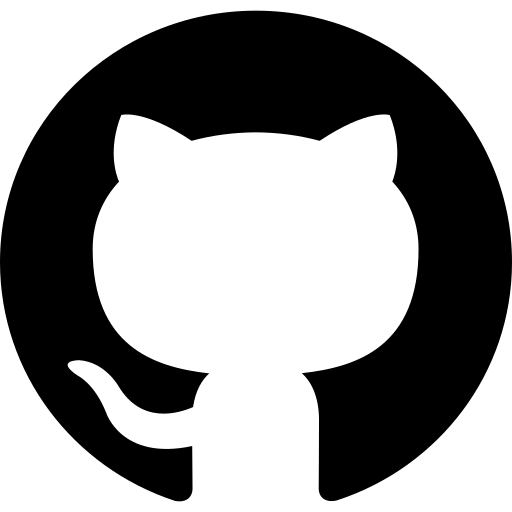
\includegraphics[width=1em]{github.png}} {\href{https://github.com/BaranGuvendiren/digital-bench-power-supply}{\texttt{GitHub Repository}}}}
\fancyfoot[C]{\thepage}

\usepackage{tabularx}
\usepackage{multirow}
\usepackage[table]{xcolor}
\renewcommand{\arraystretch}{1.4}

\usepackage[most]{tcolorbox}
\newtcolorbox{pickedbox}{
  enhanced,
  blanker,
  borderline west={1pt}{0pt}{gray!50},
  left=10pt, top=4pt, bottom=4pt
}

\usepackage{multicol}
\usepackage{tocloft}
\renewcommand{\cftsecfont}{\small\bfseries\sffamily}
\renewcommand{\cftsecpagefont}{\small\sffamily\color{blue}}
\renewcommand{\cftsubsecfont}{\small\sffamily}
\renewcommand{\cftsubsecpagefont}{\small\sffamily\color{blue}}
\renewcommand{\contentsname}{}
\renewcommand{\cftdotsep}{0.2}
\renewcommand{\cftsecleader}{\cftdotfill{\cftdotsep}}

\setlength{\cftbeforesecskip}{2pt}
\setlength{\cftbeforesubsecskip}{0pt}
\begin{document}

% Title Page
\begin{titlepage}
    \centering
    \vspace*{1.5cm}
    {\scshape\Large Hardware Design \& Verification Report \par}
    \vspace{2.5cm}
    
    {\huge\bfseries Digital Bench Power Supply \par}
    \vspace{0.4cm}
    
    {\Large\itshape Design Calculations, Circuit Simulations \& Hardware Verification \par}
    \rule{\textwidth}{1.2pt}
    
    \vspace{2.5cm}
    
    {\large\bfseries Baran Güvendiren \par}
    \vspace{0.2cm}
    {\small Electronics Engineering Student \par}

    \vfill
    \begin{minipage}{0.85\textwidth}
        \centering
        \small\itshape
        This document contains the complete theoretical calculations, simulation models, component selection justification and hardware verifications for the project.
    \end{minipage}
\end{titlepage}
\clearpage

% Table of Contents
\hypersetup{linkcolor=blue, linktoc=page}

{\centering\Large\bfseries\sffamily Table of Contents \par}
\vspace{0.25cm}

\begin{multicols}{2}
  \setcounter{tocdepth}{2}
  \tableofcontents
  \thispagestyle{fancy}
\end{multicols}
\rule{\textwidth}{0.4pt}

\hypersetup{linkcolor=black}
\clearpage

\section{Calculations \& Component Selection}
\subsection{Overview}
This section contains the theoretical calculations and engineering decisions used to determine the component values for each stage of the power supply. \\[0.5em]
The datasheet files containing manufacturer specifications and references used in these calculations are located in the \small\href{https://github.com/BaranGuvendiren/digital-bench-power-supply/tree/main/docs/datasheets}{\texttt{docs/datasheet/}} directory of the project repository. \\[1em]
{\small\itshape Note: Some calculations are based on idealized formulas with sufficient design margin to ensure system stability and flexibility in component selection. \par}

\normalsize
\subsection{Naming Convention \& Notations}
To maintain mathematical clarity across multiple stages, variables are named using the following conventions:
\begin{table}[h]
\centering
\caption{Naming Convention}
\label{tab:convention}
\small
\begin{tabularx}{\textwidth}{|l|>{\raggedright\arraybackslash}X|l|}
\hline
\rowcolor{gray!20} 
\textbf{Notation Format} & \textbf{Description}               & \textbf{Example} \\ \hline
No Parentheses           & Global board-level variable        & $\mathrm{V_{OUT}}$ (Board output voltage) \\ \hline
With Parentheses         & Component specific to a certain IC & $\mathrm{V_{OUT(U1)}}$ (Output voltage specific to U1 - LM25117) \\ \hline
\end{tabularx}
\end{table}

{\small\itshape Note: The number inside the parentheses indicates which integrated circuit (IC) the variable belongs to. \par}

\begin{table}[h]
\centering
\caption{IC Reference Table}
\label{tab:notations}
\small
\begin{tabularx}{\textwidth}{|c|c|>{\raggedright\arraybackslash}X|}
\hline
\rowcolor{gray!20} 
\textbf{IC Number} & \textbf{Component Name} & \textbf{Description} \\ \hline
1                  & LM25117                 & Main Buck Pre-Regulator \\ \hline
2                  & MIC29302                & Main LDO \\ \hline
4                  & TPS54331                & Auxiliary 5 V Buck Regulator \\ \hline
6                  & TPS54332                & Auxiliary 12 V Buck Regulator \\ \hline
\end{tabularx}
\end{table}

\subsection{LM25117 - U1}
\subsubsection{Timer Resistor \texorpdfstring{$\mathrm{R_{T(U1)}}$}{RT(U1)}}
The switching frequency of the main buck regulator was set to \qty{\fswA}{\hertz} via the $\mathrm{R_{T(U1)}}$ pin resistor; 
this enables sufficient separation from the adapter's lower switching frequency ($\approx \qty{100e3}{\hertz}$) to minimize beat frequency noise, while preventing excessive switching losses at higher frequencies.
\begin{align}
\mathrm{R_{T(U1)}} &= \frac{\num{5.2e9}}{\mathrm{f_{SW(U1)}}} - 949 \nonumber \\[0.5em]
                   &= \frac{\num{5.2e9}}{\num{\fswA}} - 949 \approx \qty{\CalcRtA}{\ohm}
\end{align}
\begin{pickedbox}
\small\textbf{Picked Value(s):}\\[0.5em]
$\diamond\quad \mathrm{R_{T(U1)}} = \qty{\RtA}{\ohm}$
\end{pickedbox}

\subsubsection{Output Inductor \texorpdfstring{$\mathrm{L_{O(U1)}}$}{LO(U1)}}
The output inductance was calculated using a nominal mid-range voltage of $\mathrm{V_{OUT(TYP)}} = \qty{\VoutTyp}{\volt}$ to achieve a balanced ripple current trade-off over the full output voltage range. 
In addition, maximum inductor ripple ($\mathrm{I_{PP(U1)}}$) current was selected as \qty{20}{\percent} of the full load current.
\begin{align}
\mathrm{L_{O(U1)}} &= \frac{\mathrm{V_{OUT(TYP)}}}{\mathrm{I_{PP(U1)}} \cdot \mathrm{f_{SW(U1)}}} \cdot \left(1 - \frac{\mathrm{V_{OUT(TYP)}}}{\mathrm{V_{IN}}}\right) \nonumber  \\[0.5em]
                   &= \frac{\VoutTyp}{\IppA \cdot \num{\fswA}} \cdot \left(1 - \frac{\VoutTyp}{\Vin}\right) \approx \qty{\CalcLoA}{\henry}
\end{align}
\begin{pickedbox}
\small\textbf{Picked Value(s):}\\[0.5em]
$\diamond\quad \mathrm{L_{O(U1)}} = \qty{\LoA}{\henry}$
\end{pickedbox}

\subsubsection{Current Sense Resistor \texorpdfstring{$\mathrm{R_{CS(U1)}}$}{RCS(U1)}}
Maximum output current capability ($\mathrm{I_{OUT(MAX)}}$) was selected as \qty{150}{\percent} of the full load current to account for tolerances. \\[1em]
{\small\itshape Note: Since the LM25117 uses an emulated current ramp, it reads the valley current just before the high-side switch turns on. This means the controller is unaffected by the large leading-edge switching spikes. 
Therefore, a current sense filter was not used in this design to avoid propagation delay on current sensing. \par}
\begin{align}
\mathrm{R_{CS(U1)}}  &= \frac{\mathrm{V_{CS(TH)}}}{\mathrm{I_{OUT(MAX)}} + \dfrac{\mathrm{V_{OUT(TYP)}} \cdot \mathrm{K}}{\mathrm{f_{SW(U1)}} \cdot \mathrm{L_{O(U1)}}} - \dfrac{\mathrm{I_{PP(U1)}}}{2}} \nonumber \\[0.5em]
                     &= \frac{0.12}{\num{\IoutMax} + \dfrac{\num{\VoutTyp} \cdot 1}{\num{\fswA} \cdot \num{\LoA}} - \dfrac{\num{\IppA}}{2}} \approx \qty{\CalcRcsA}{\ohm}\\[1.5em]
\mathrm{P_{RCS(U1)}} &= \left(1 - \frac{\mathrm{V_{OUT(MIN)(U1)}}}{\mathrm{V_{IN}}}\right) \cdot \mathrm{I_{OUT}}^2 \cdot \mathrm{R_{CS(U1)}} \nonumber \\[0.5em]
                     &= \left(1 - \frac{\num{\VoutMin}}{\num{\Vin}}\right) \cdot \num{\Iout}^2 \cdot \num{\RcsA} \approx \qty{\PrcsA}{\watt}
\end{align}
\begin{pickedbox}
\small\textbf{Picked Value(s):}\\[0.5em]
$\diamond\quad \mathrm{R_{CS(U1)}} = \qty{\RcsA}{\ohm}$ \\[0.25em]
$\diamond\quad \mathrm{P_{RCS(U1)}} = \text{[TBD]}$  % \qty{\Prcs}{\watt}
\end{pickedbox}

\subsubsection{Ramp Resistor and Capacitor \texorpdfstring{$\mathrm{R_{RAMP(U1)}}$ and $\mathrm{C_{RAMP(U1)}}$}{CRAMP(U1)}}
Current sense amplifier gain ($\mathrm{A_{RAMP}}$) and K factor are both defined in the datasheet. K factor was set to 1 to prevent sub-harmonic oscillations and ensure one-cycle damping, as recommended in the datasheet. \\[1em]
{\small\itshape Note: The value of $\mathrm{C_{RAMP(U1)}}$ was set to the standard capacitor value of 1 nF. \par}
\begin{align}
\mathrm{R_{RAMP(U1)}} &= \frac{\mathrm{L_{O(U1)}}}{\mathrm{K} \cdot \mathrm{C_{RAMP(U1)}} \cdot \mathrm{R_{CS(U1)}} \cdot \mathrm{A_{RAMP}}} \nonumber \\[0.5em]
                      &= \frac{\num{\LoA}}{1 \cdot \num{\CrampA} \cdot \num{\RcsA} \cdot 10} = \qty{\CalcRrampA}{\ohm}
\end{align}
\begin{pickedbox}
\small\textbf{Picked Value(s):}\\[0.5em]
$\diamond\quad \mathrm{R_{RAMP(U1)}} = \qty{\RrampA}{\ohm}$ \\[0.25em]
$\diamond\quad \mathrm{C_{RAMP(U1)}} = \qty{\CrampA}{\farad}$
\end{pickedbox}

\subsubsection{Output Shunt Resistor \texorpdfstring{$\mathrm{R_S}$}{RS}}
The output current was measured by converting the load current ($\mathrm{I_{OUT(U1)}}$) into an analog voltage signal via a dedicated shunt resistor and a current sense amplifier. The resulting analog signal was then digitized by the MCU's ADC. 
Since the LDO's input current is approximately equal to its output current, the shunt resistor was placed before the feedback node at the LDO input to prevent the voltage drop across the shunt resistor from affecting the regulated output voltage. \\[0.5em]
As low power consumption was not a primary concern for this project, the amplifier gain ($\mathrm{A_S}$) was set to \qty{50}{\times} to minimize the amplification of measurement errors. 
In addition, the reference voltage ($\mathrm{V_{S(REF)}}$) was limited to \qty{3}{\volt}, providing \qty{0.3}{\volt} headroom below the MCU supply voltage to reduce the impact of possible control errors. \\[1em]
{\small\itshape Note: $R_{CS(U1)}$ was used to measure the inductor valley current for LM25117's emulated current-mode control, while $R_S$ was used to calculate the output current for monitoring and setting CC-mode current limit. \par}
\begin{align}
\mathrm{R_S}    &= \frac{\mathrm{V_{S(REF)}} / \mathrm{A_S}}{\mathrm{I_{OUT}}} \nonumber \\[0.5em] 
                &= \frac{\TargVsRef / \As}{\Iout} \approx \qty{\CalcRs}{\ohm} \\[1.5em]
\mathrm{P_{RS}} &= \mathrm{I_{OUT}}^2 \cdot \mathrm{R_S} \nonumber \\[0.5em]
                &= \num{\Iout}^2 \cdot \num{\Rs} \approx \qty{\CalcPrs}{\watt}
\end{align}
\begin{pickedbox}
\small\textbf{Picked Value(s):}\\[0.5em]
$\diamond\quad \mathrm{R_S} = \qty{\Rs}{\ohm}$ \\[0.25em]
$\diamond\quad \mathrm{P_{RS}} = \text{[TBD]}$  % \qty{\Prs}{\watt}
\end{pickedbox}
\end{document}